\documentclass[12pt,a4paper]{report}
\usepackage[spanish]{babel}
\usepackage{csquotes, graphicx, subcaption, url, multicol}
\renewcommand{\chaptername}{Capitulo}
\title{Implatación de técnicas y herramientas de pentesting en el proceso de desarrollo de software}
\author{Emilio J Roldán}

\usepackage[backend=biber,style=verbose-note]{biblatex}
\usepackage[colorlinks=true, allcolors=blue]{hyperref}

\addbibresource{bibliografia.bib} 
% Load the package
\usepackage[toc,section,automake]{glossaries}
 
% Generate the glossary
\makeglossaries
\loadglsentries{glosario}


\begin{document}

\maketitle
\tableofcontents

% list of tables
%\listoftables
%\addcontentsline{toc}{chapter}{List of Tables}

% list of figures
%\listoffigures
%\addcontentsline{toc}{chapter}{List of Figures}
\newpage

\chapter{Introducción.}
\chapter{Introducción.}
\section{motivación y objetivos}

  El motivo principal que me ha llevado a realizar este proyecto es relatar como realizar un proceso 
de pentesting resaltando dos herramientas que a día de hoy hay muchos pentester que no suelen utilizar
como son los análisis de código, sobre todo la parte estática, así como la integración de dichas 
pruebas en el ciclo de desarrollo Software.

\clearpage

\chapter{Análisis del estado del arte}
\input{chapters/02_Análisis del estado del arte.tex} 
 
\chapter{Diseño solución técnica.}

\input{./chapters/031_MétodologiaPruebas.tex}

\section{Infraestructura de pruebas} 
Como entorno de pruebas para la ejecución de los análisis de código; haremos uso de una máquina física y de un contenedor 
de Docker con la siguientes características y herramientas instaladas en cada una de ellas:

\begin{table}[!htb]
    \begin{center}
      \begin{tabular}{c| c |c}
      \hline 
        \rowcolor{tema!10}
        \bft{Características} & \bft{Máquina física} & \bft{Contenedor}\\
        \hline
        Sistema Operativo & Windows 10 Pro & Debian GNU/Linux 10 (buster)\\  \hline
        \multirow{3}{4em}{Herramientas} & OWASP Zap 2.10 & SonarQube 8.2 \\
        & Dependency-check & PostGresSQL 13.3 \\ 
        & SonarScaner 4.6.2 &  \\ \hline
      \end{tabular}
      \caption{Infraestructura de pruebas}
      \label{tab:InfraestructuraPruebas}
    \end{center}
  \end{table}

Para levantar el contenedor podemos hacer uso de dockercompose incluido en la carpeta \textbf{"entornoPrueba"} dentro de 
las \href{https://github.com/M0l1n3ta/PFG/tree/master}{fuentes de proyecto}

Para levantar el entorno ejecutamos:\\

\begin{verbatim}
    docker-compose up
\end{verbatim}

\begin{figure}[!htb]
    \centering
    \captionsetup{width=1\linewidth}    
    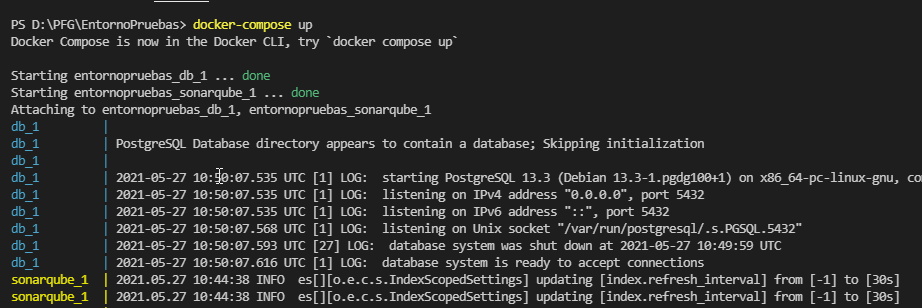
\includegraphics[width=\linewidth]{./imagenes/04_DockerCompose_UP.png}
    \caption{Docker compose up}  
\end{figure}

\clearpage
\newpage
Una vez que se veamos las siguientes líneas en el log:\\
\begin{figure}[!htb] 
    \captionsetup{width=1\linewidth}   
    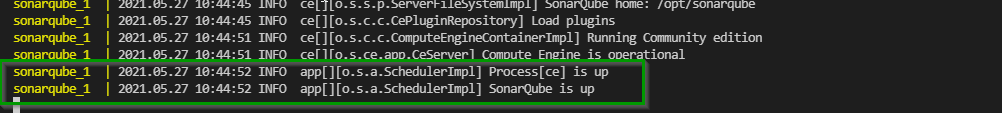
\includegraphics[width=\linewidth]{./imagenes/05_SonarQubeServerRunning.png}
    \caption{SonarQube server running}  
\end{figure}

Podremos acceder a la página de SonarQube en 
la url \href{http://localhost:9000}{http://localhost:9000}\\
\begin{figure}[!htb] 
    \captionsetup{width=1\linewidth}   
    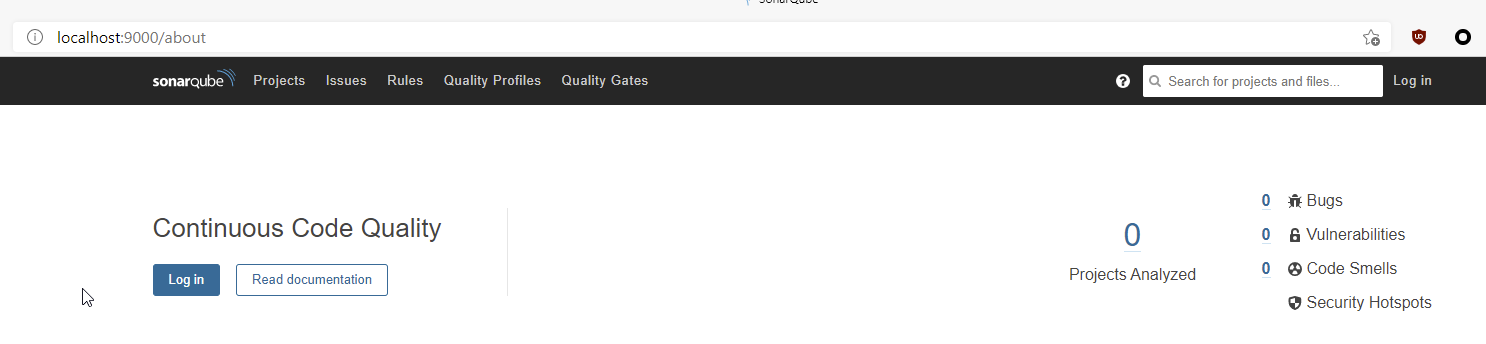
\includegraphics[width=\linewidth]{./imagenes/06_SonarQubeServer_Webpage.png}
    \caption{SonarQube portal}  
    \label{fig:21}
\end{figure}

\clearpage
\newpage
El fichero del docker compose \ref{alg:dockercompose} muestra los componentes de a aquitectura utilizados:

\begin{listing}
    \centering
    \inputminted{yaml}{./EntornoPruebas/SonarQube_8.2/docker-compose.yml}
    \caption{Docker Compose}
    \label{alg:dockercompose}
\end{listing}

\clearpage

\chapter{Ejecución casos de prueba.}
\section{Aplicación en desarrollo de aplicaciones Web} 

Como aplicaciones para los casos de prueba haremos uso de las siguientes aplicaciones:

\begin{table}
    \begin{center}
      \caption{Parámetros línea comandos dependency-check}
      \label{tab:tabla 2}
      \begin{tabular}{c|c}
        \textbf{Aplicación} & \textbf{Tecnologías utilizadas}\\
        \hline
        \href{https://dvwa.co.uk/}{Damn Vulnerable Web application (dwva)} & PHP\\ 
        \href{https://github.com/bkimminich/juice-shop}{Juice Shop} & JavaScript, Angular, Node.js\\
        \href{https://github.com/WebGoat/WebGoat}{WebGoat} &  Java, Spring Boot\\
        \href{https://github.com/tobyash86/WebGoat.NET}{WebGoat.Net} & .Net Core     
      \end{tabular}
    \end{center}
  \end{table}

\subsubsection{Damn Vulnerable Web application (DVWA)}

Siguiendo las tareas del \href{https://github.com/M0l1n3ta/PFG/blob/master/Reportes/DVWA/PPR DVWA - Plan Pruebas de Seguridad.docx}{documento de plan pruebas}
para este proyecto, realizamos las tareas que se detallan a continuación.

Para este proyecto no se realizará análisis de dependencias puesto que el proyecto no hace uso del componente de PHP 
necesario para realizar este tipo de análisis en proyectos PHP (\href{https://getcomposer.org/}{Composer})

La ejecución del análisis estático de código lo realizaremos a través de un
\href{https://github.com/M0l1n3ta/PFG/blob/master/Scripts/STAT/RunSonarScaner_DWVA.ps1}{script}, con el cual obtenemos 
el siguiente resultado:

\begin{figure}[h!]  
    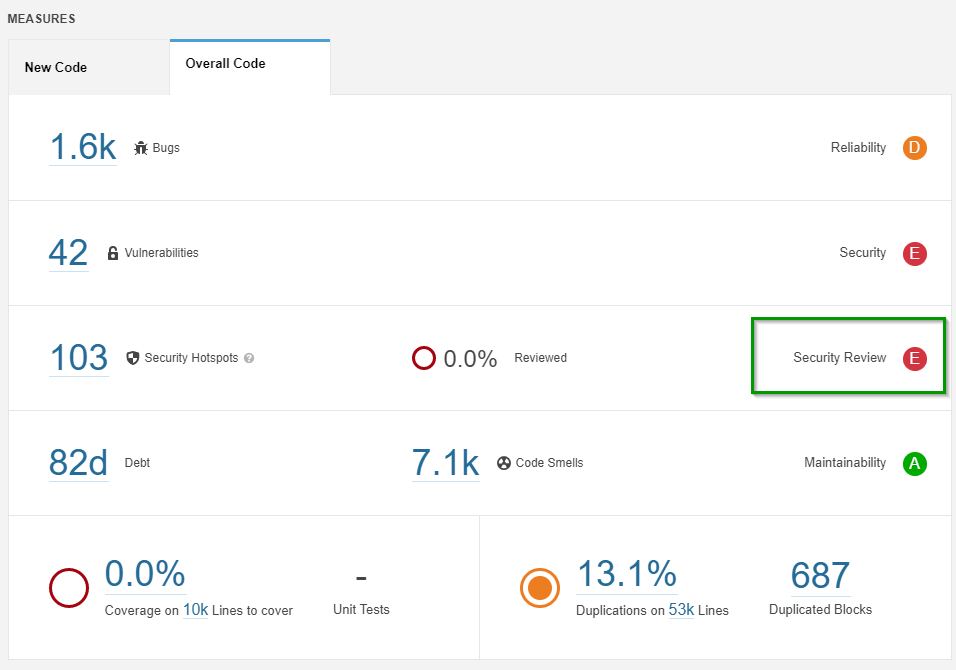
\includegraphics[width=\linewidth]{./imagenes/07_AnalisisEstatico__DVWA.png}
    \caption{Resultado análisis estatico código DVWA}  
    \label{fig:7}
\end{figure}
Como era de esperar obtiene el peor resultado posible en la medida de seguridad \textbf{“E”}

\subsubsection{Juice Shop}
Siguiendo las tareas del documento de plan pruebas para este proyecto, realizamos las tareas que se detallan a continuación.
La ejecución del análisis estático de código, así como el análisis de dependencias, lo realizaremos a través de un 
\href{https://github.com/M0l1n3ta/PFG/blob/master/Scripts/STAT/RunSonarScaner_JuiceShop.ps1}{script}, con el cual obtenemos 
el siguiente resultado:

\begin{figure}[h!]  
    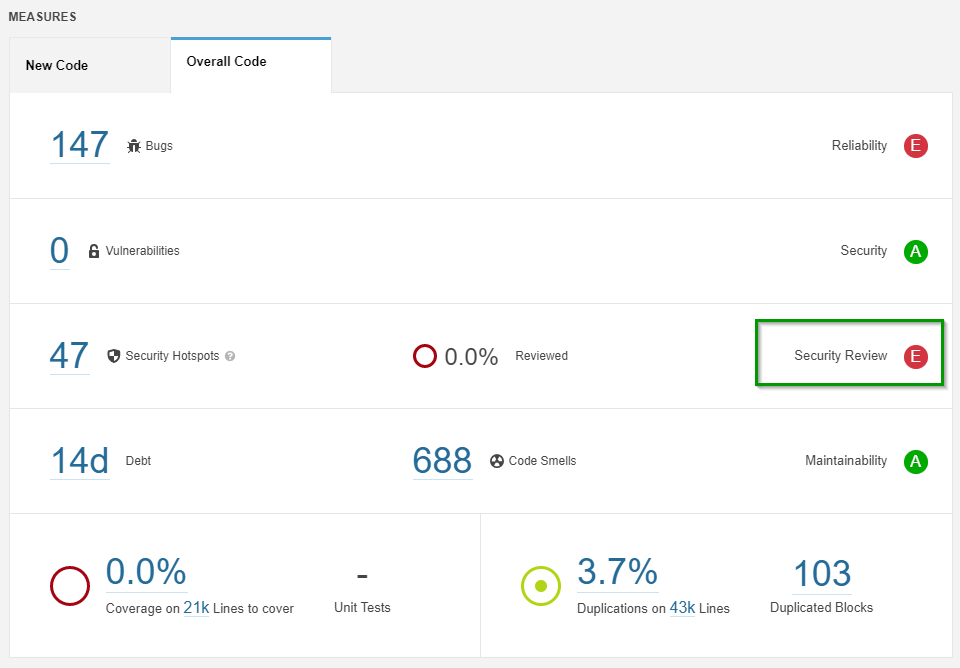
\includegraphics[width=\linewidth]{./imagenes/08_AnalisisEstatico_JuiceShop.png}
    \caption{Resultado análisis estatico código Juice Shop}  
    \label{fig:8}
\end{figure}
Como era de esperar obtiene el peor resultado posible en la medida de seguridad \textbf{“E”}

\subsubsection{WebGoat}
Siguiendo las tareas del documento de plan pruebas para este proyecto, realizamos las tareas que se detallan a continuación.

Para ejecutar el análisis de dependencias desde Maven, debemos añadir la siguiente configuración del plugin de Dependency-Check:

\begin{listing}[ht]
    \inputminted{xml}{./Ficheros/ConfiguracionPlugin_Maven.xml}
    \caption{Example from external file}
    \label{listing:4}
\end{listing}
A parte de la configuración anterior debemos añadir las siguientes propiedades:
\begin{listing}[ht]
    \inputminted{xml}{./Ficheros/ConfigPropertiesPlugin_maven.xml}
    \caption{Example from external file}
    \label{listing:4}
\end{listing}
Para ejecutar el escáner
\begin{verbatim}
    mvn dependency-check:check
\end{verbatim}

La ejecución del análisis estático de código, así como el análisis de dependencias, lo realizaremos a través de un 
\href{https://github.com/M0l1n3ta/PFG/blob/master/Scripts/STAT/RunSonarScaner_WebGoat.ps1}{script}, con el cual
obtenemos el siguiente resultado:
\begin{figure}[h!]  
    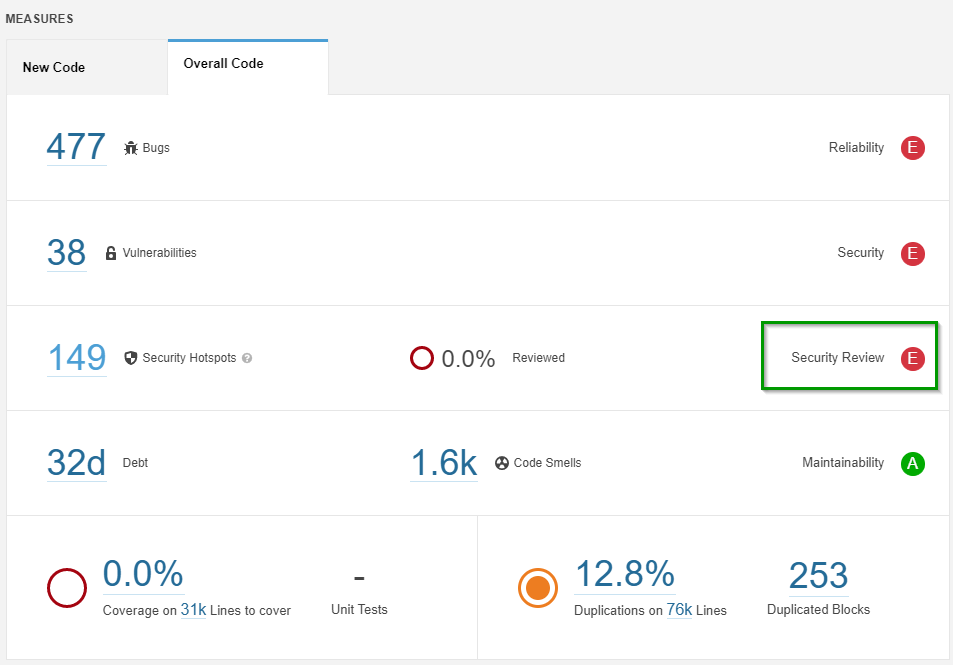
\includegraphics[width=\linewidth]{./imagenes/09_AnalisisEstatico_WebGoat.png}
    \caption{Resultado análisis estatico código WebGoat}  
    \label{fig:9}
\end{figure}
Como era de esperar obtiene el peor resultado posible en la medida de seguridad \textbf{“E”}

\subsubsection{WebGoat.Net}
Siguiendo las tareas del documento de plan pruebas para este proyecto, realizamos las tareas que se detallan a continuación.

La ejecución del análisis estático de código, así como el análisis de dependencias, lo realizaremos a través de un 
\href{https://github.com/M0l1n3ta/PFG/blob/master/Scripts/STAT/RunSonarScaner_WebGoat.NET.ps1}{script}, con el cual obtenemos
el siguiente resultado:
\begin{figure}[h!]  
    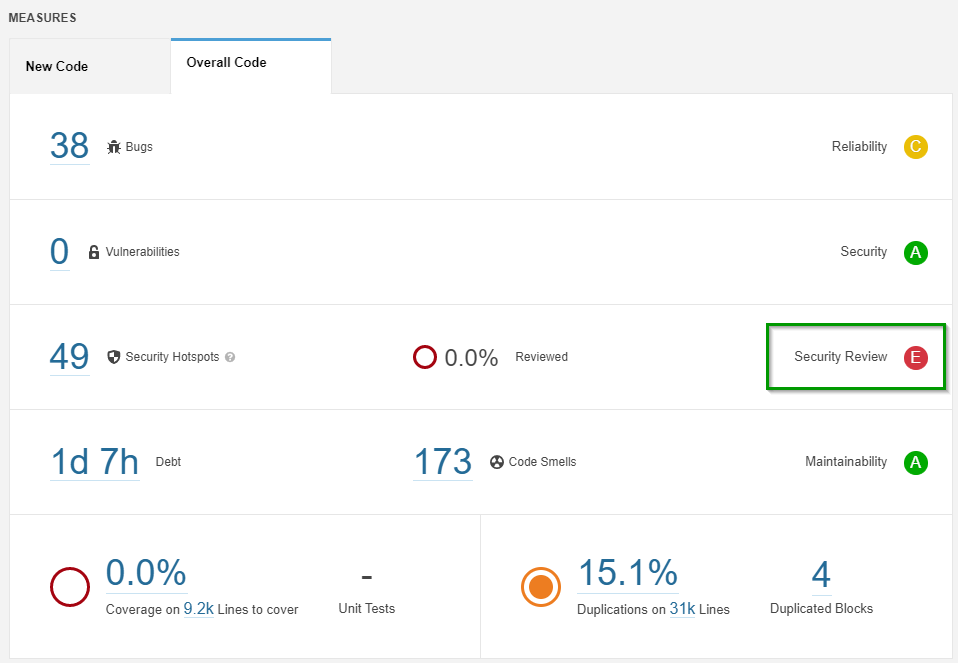
\includegraphics[width=\linewidth]{./imagenes/10_AnalisisEstatico_WebGoat.Net.png}
    \caption{Resultado análisis estatico código WebGoat}  
    \label{fig:9}
\end{figure}
Como era de esperar obtiene el peor resultado posible en la medida de seguridad \textbf{“E”}

\section{Aplicación en desarrollo de Servicios Web} 



\newpage
\addcontentsline{toc}{section}{Bibliografia}
\printbibliography[title=Bibliografia]

%Print the glossary
\printglossaries

\end{document}